\documentclass{article}

\usepackage[margin=1in]{geometry}
\usepackage{amsmath, amsthm}
\usepackage{float}
\usepackage{graphicx}
\usepackage{listings}
\usepackage{color}
\title{Exploratory Flux Predictions}
\author{Nicholas Kaufman}

\begin{document}
\maketitle

This report will detail the results of predicting average flux emissions using three different models.

\section*{Random Forests}

\subsection*{The First Model}
For the first model, time was eliminated as a training variable. All other factor variables - Air Temperature, three layers of Soil Temperature, Soil Moisture, and Light - were used.

A plot is included below showing some preliminary results.

\begin{figure}[H]
	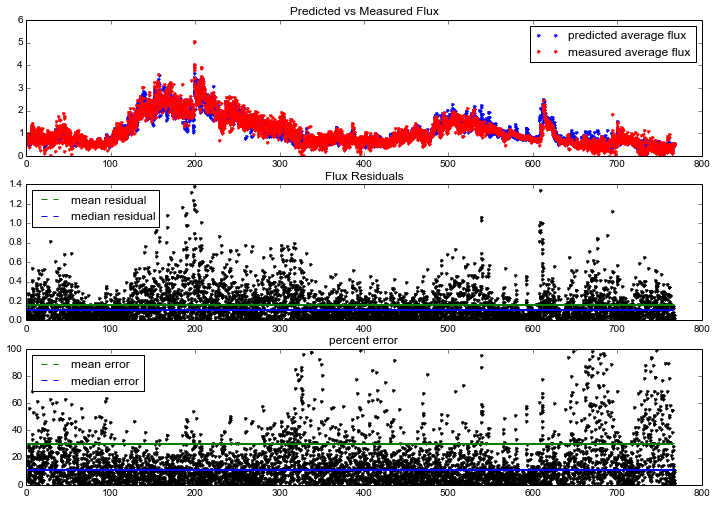
\includegraphics[width=\textwidth, height=\textheight, keepaspectratio]{rf1.png}
\end{figure}

While training, the R2 score (or the coefficient of determination) is calculated on the training data, and on a cross-validation set. Those values are given below: \\
R2 score on training data:  0.982474990177 \\
R2 score on 5-folded data:  [0.87108384  0.87205808  0.86948272  0.86920592  0.85897424] \\
Average score across folds:  0.868160959768 \\

R2 obtains a maximum at 1, and is a measure of how well the model is performing on a particular data set, for which we can compare a known baseline. \\

One can also compute the weights the model gives to each of the feauture variables. In this case, those are: \\

Featrure Importance Vector: [0.04442861  0.59248679  0.0466869   0.03521874  0.25649003  0.02468893] \\

The higher the number, the more important the weight. From this we see that, by a large margin, the deepest soil temperature and light are the most important features. \\

It is interesting to note that, in the predictions plot above, we can see two time distinct time periods in which the models performance is weakest. It is also worthy of mention that since this data is over the span of two years, those areas appear to correspond to roughly the same yearly time range. We can conclude that perhaps it would be useful to include the time as a variable. \\

In order to present a perhaps cleaner picture, we include the same plots but using only every tenth data point.

\begin{figure}[H]
	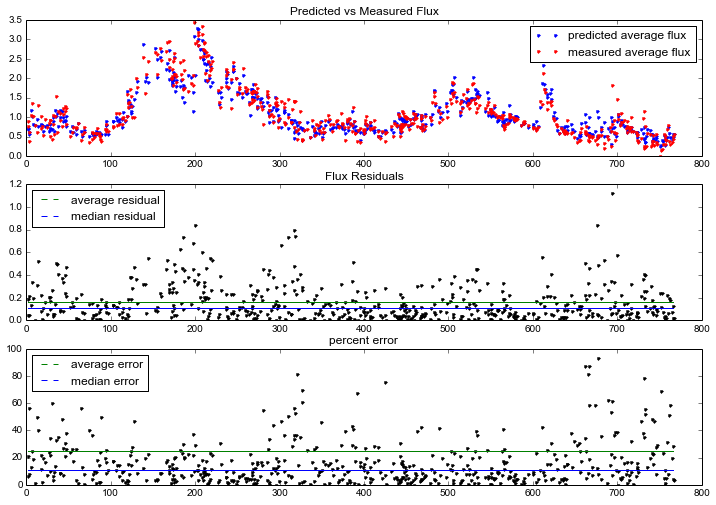
\includegraphics[width=\textwidth, height=\textheight, keepaspectratio]{rf1_small.png}
\end{figure}

\subsection*{The Second Model}
Here we include time as a variable, according to the discussion following the previous plot. When training the model with this additional factor variable, the predictions improve.

\begin{figure}[H]
	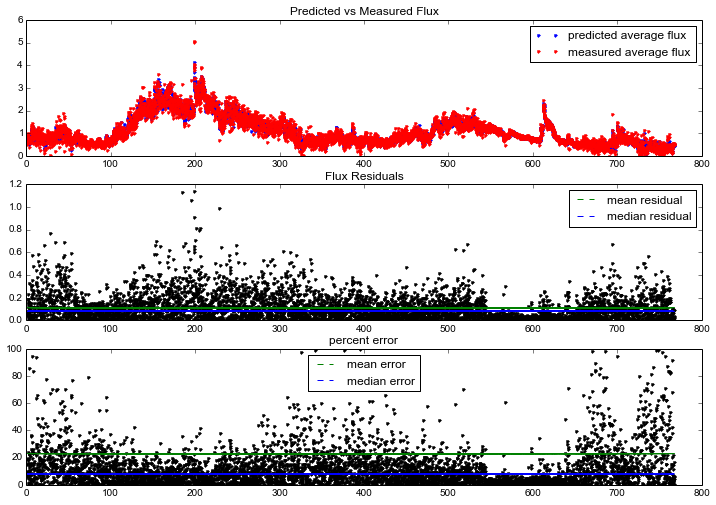
\includegraphics[width=\textwidth, height=\textheight, keepaspectratio]{rf2.png}
\end{figure}

We notice that the predictions are significantly more accurate here. We include the calculated output as before.

R2 score on training data:  0.990912535056
R2 score on 5-folded data:  [ 0.9345659   0.93356225  0.93235294  0.9353663   0.92977682]
Average score across folds:  0.933124842167

R2 score on testing data:

Feature Importance Vector: [0.02230462  0.50997696  0.01256326  0.01180546  0.05988339  0.00664382 0.37682248] \\

From this, we see that light is now no longer an important feature. Time as taken it's place by a large margin as the penultimate feature.

Again, we plot the results using a tenth of the data for a neater picture.

\begin{figure}[H]
	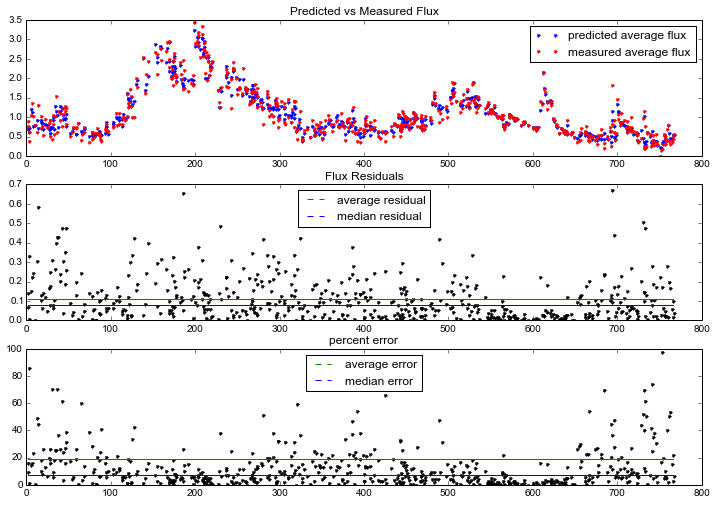
\includegraphics[width=\textwidth, height=\textheight, keepaspectratio]{rf2_small.png}
\end{figure}

\section{Support Vector Machine}

\subsection{The Third Model}

This model's performance is quite inferior to the previous models. The results are included because they highlight the importance of time as a variable. Note that it is impossible to use time as a variable in SVM models because the model requires the data to be scaled to fit the Standard Distribution, per feature. This is obviously infeasible to do with time.

\begin{figure}[H]
	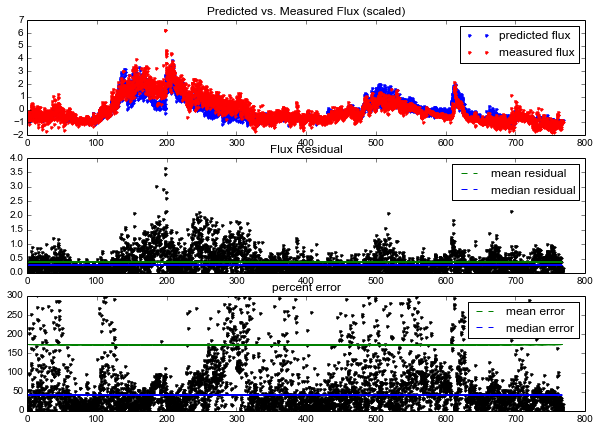
\includegraphics[width=\textwidth, height=\textheight, keepaspectratio]{svm1.png}
\end{figure}

Here we can very clearly see the two regions in time in which the prediction most notably breaks down. I believe that given more feature variables, we can highlight which attributes are most significant in predicting the average flux. Further, I believe that it would be possible to use similar methodologies to predict the amount of flux for varying gasses based on a larger range of dependent variables.

\section{Source Code}
\lstset{language=Python, numbers=left, frame=shadowbox, rulesepcolor=\color{blue}}
\lstinputlisting{flux_prediction.py}

\end{document}